\chapter{Исследовательская часть}

Замеры выполнялись на микроконтроллере STM32, со следующими характеристиками~\cite{stm32}:
\begin{itemize}[label=---]
	\item 32-битный процессор архитектуры ARM с частотой 256 МГц;
	\item оперативная память: 512 Кбайт.
\end{itemize}

\section{Замеры процессорного времени}

Для замеров использовались случайно сгенерированные строки длинной до 10 символов. Для каждой пары строк совпадающей длины замеры проводились 50 раз. Замеры проводились с  помощью функции micros()~\cite{micros}. В таблице~\ref{tab:all_times} представлены результаты замеров.

\begin{table}[H]
	\caption{Результаты замеров времени для различных реализаций алгоритмов поиска и длин входных строк в секундах для 50 запусков}
	\centering
	\begin{tabular}{|c|r|r|r|r|}
		\hline
		\multirow[c]{2}{*}{\shortstack{Длины\\строк}} &
		\multicolumn{3}{|c|}{\shortstack{Расстояние\\ Левенштейна}} & \multicolumn{1}{c|}{\shortstack{Расстояние\\ Дамерау---Левенштейна}} \\
		\hhline{|~|-|-|-|-|}
		& \multicolumn{1}{|c|}{\shortstack{Рекурсивная\\ реализация}} & \multicolumn{1}{c|}{\shortstack{\shortstack{Рекурсивная\\ реализация}\\ с мемоизацией}} & \multicolumn{1}{c|}{\shortstack{Итеративная\\ реализация}}& \multicolumn{1}{c|}{\shortstack{Итеративная\\ реализация}}\\
		\hline
		1 & 0.000009 & 0.000033 & 0.000059 & 0.000086\\
		\hline
		2 & 0.000041 & 0.000059 & 0.000058 & 0.000074\\
		\hline
		3 & 0.000186 & 0.000180 & 0.000062 & 0.000088\\
		\hline
		4 & 0.000968 & 0.000729 & 0.000074 & 0.000098\\
		\hline
		5 & 0.005069 & 0.003389 & 0.000073 & 0.000105\\
		\hline
		6 & 0.028604 & 0.020497 & 0.000081 & 0.000083\\
		\hline
		7 & 0.133681 & 0.113024 & 0.000089 & 0.000098\\
		\hline
		8 & 0.696408 & 0.501769 & 0.000099 & 0.000108\\
		\hline
		9 & 3.987760 & 2.801120 & 0.000123 & 0.000119\\
		\hline
		10 & 23.923900 & 12.220100 & 0.000156 & 0.000123\\
		\hline
	\end{tabular}
	\label{tab:all_times}
\end{table}


На рисунке~\ref{fig:all_lev_plots} представлены графики замеров времени для каждой из трех реализаций алгоритма поиска расстояния Левенштейна.
\begin{figure}[H]
	\centering
	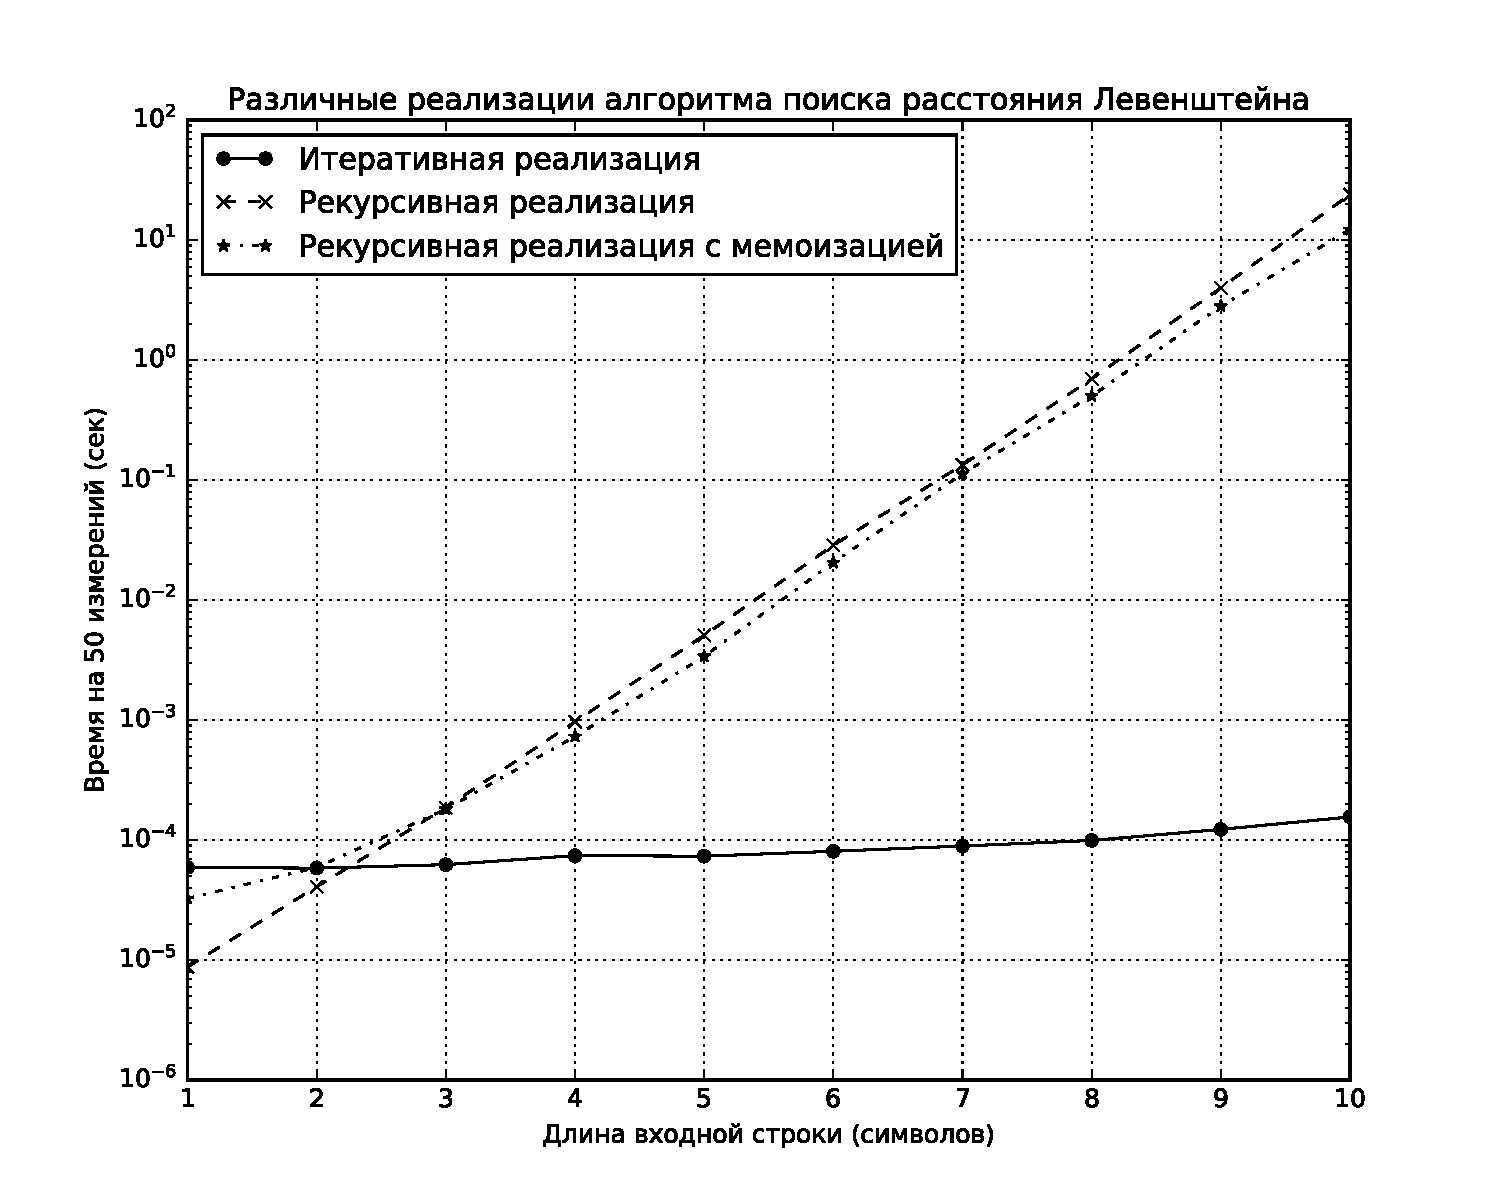
\includegraphics[width=\textwidth]{all_lev.pdf}
	\caption{Графики замеров времени для представленных реализаций поиска расстояния Левенштейна}
	\label{fig:all_lev_plots}
\end{figure} 

На рисунке~\ref{fig:lev_dam_lev_plots} представлены графики замеров времени для итеративных реализаций алгоритмов поиска расстояний Левенштейна и Дамерау---Левенштейна.
\begin{figure}[H]
	\centering
	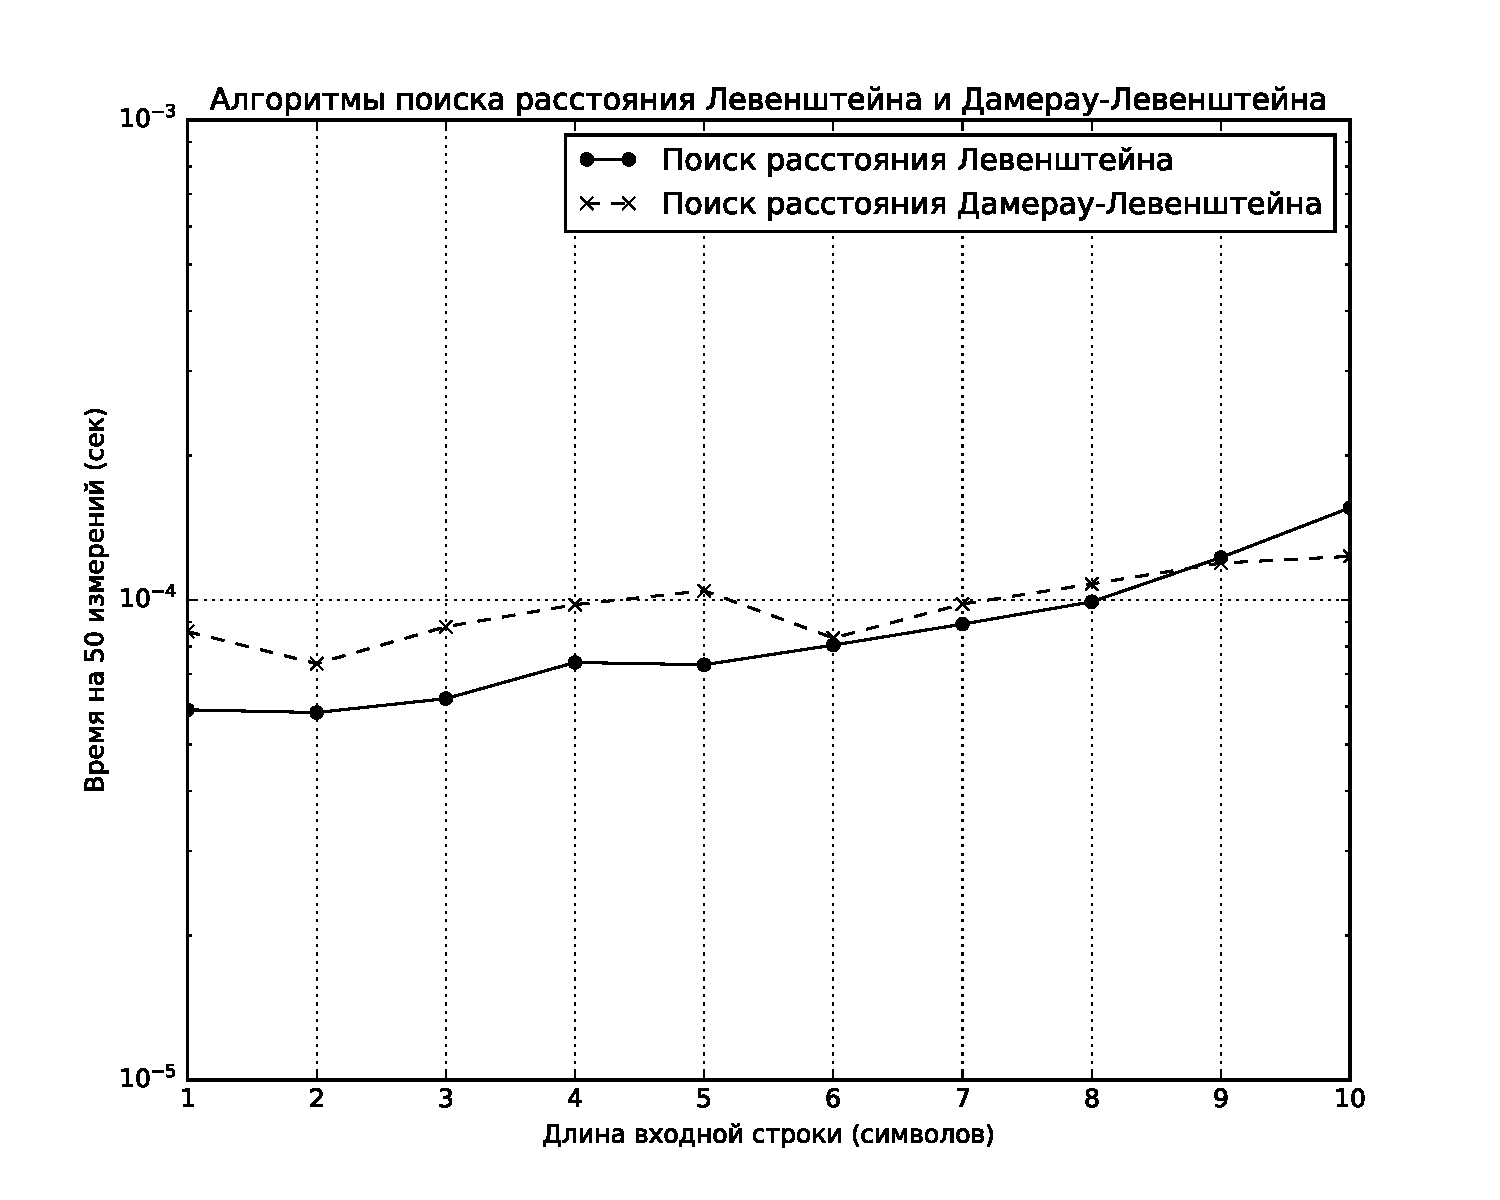
\includegraphics[width=\textwidth]{lev_vs_dam_lev.pdf}
	\caption{Графики замеров времени для итеративных алгоритмов поиска расстояний Левенштейна и Дамерау---Левенштейна}
	\label{fig:lev_dam_lev_plots}
\end{figure} 

\section{Оценка емкостных затрат}

Для итеративных реализаций алгоритмов поиска редакционных расстояний оценка складывается из размера выделенной матрицы и некоторых дополнительных константных затрат:
\begin{itemize}[label=---]
	\item для алгоритма поиска расстояния Левенштейна 
	\begin{equation}
		2\cdot min(n, m) + 2\cdot 4 + 2 \cdot 4 + 2 \cdot 4 = 2 \cdot min(n, m) + 24 \approx O(n)
	\end{equation}
	где\begin{itemize}
		\item $2\cdot min(n, m)$ --- для хранения матрицы уже рассчитанных значений;
		\item $2\cdot 4$ --- для хранения размеров входных строк
		\item $2\cdot 4$ --- для хранения указателей в матрице значений
		\item $2\cdot 4$ --- для хранения счетчиков циклов
	\end{itemize}
	\item для алгоритма поиска расстояния Дамерау---Левенштейна
	\begin{equation}
		3\cdot min(n, m) + 2\cdot 4 + 3 \cdot 4 + 2 \cdot 4 = 2 \cdot min(n, m) + 28 \approx O(n)
	\end{equation}
	где слагаемые указаны аналогично предыдущему случаю
\end{itemize}

В рекурсивной реализации каждый вызов делает три рекурсивных вызова. Считая для оценки дерево полным, его высота $h = max(n, m)$. При этом, так как вызовы осуществляются последовательно, единовременно в стеке не более $h$ вызовов. Каждый вызов принимает копии подстрок, то есть еще $2 \cdot max(n, m)$ памяти. Таким образом итоговая оценка $h \cdot 2 \cdot max(n, m) = 2 \cdot max(n, m)^2 = O(n^2)$.
\section{Вывод}
Рекурсивные реализации в среднем медленнее итеративных. Рекурсивная реализация алгоритма с мемоизацией быстрее, чем та же реализация без нее, так как избавляет от повторных вызовов для тех же входных значений.

Итеративная реализация алгоритма поиска расстояния Дамерау---Левенштейна медленнее, чем такая же для поиска расстояния Левенштейна в связи с необходимостью учета операции транспозиции и дополнительных связанных с этим проверок.

По памяти итеративные реализации эффективнее рекурсивных.


\clearpage